\chapter{State of the Art}

This chapter will outline the current state-of-the-art research surrounding carbon aware (temporal) scheduling, as well as the approach taken for determining that.

\paragraph{Systematic Approach}

We used the following system for finding related work to my topic.
First, two groups of keywords are brainstormed for use in querying academic search engines, one group corresponds to carbon-awareness and the other deals with computing environments.
The specific keywords used for each group are listed in Table \ref{tab:lit_study_keywords}.

\begin{table}[h!]
\centering
\begin{tabular}{|c|p{7cm}|}
\hline
    Group & Keywords \\ \hline
    carbon-awareness & \text{energy efficiency}, \text{energy consumption}, \text{carbon impact} \\ \hline
    \text{computing environments} & \text{datacenter}, \text{load balancing}, \text{scheduling}, \text{job shop}, \text{job management}, \text{compute cluster}, \text{hpc}, \text{placement}, \text{cloud} \\ \hline
\end{tabular}
\caption{List of keywords for each group used in the literature study}
\label{tab:lit_study_keywords}
\end{table}

Using these two groups, I could then create Google Scholar queries via the cross product between them. 
Use of the double-quotation feature restricts the results further.
For each query, we then read the abstracts of, on average, the first 5 results, depending on if their titles seemed subjectively fit. 

These are then be entered into a spreadsheet: for each query, 5 paper titles. Additionally, we further explored papers through \emph{connected papers}\footnote{\url{https://www.connectedpapers.com/}} or looking up individual authors on a subjective basis. 
The papers from the 2023 and 2024 HotCarbon Workshops\footnote{\url{https://hotcarbon.org/}} also proved to be related.

We then sort each paper into one of the following category:

\begin{itemize}
    \item Green, meaning that they seem very connected and are good first entries into the topic
    \item Orange indicates that are somehow connected to the paper and might be read at a later date
    \item Red, the paper is either irrelevant or had some other flaw. These will not be used again in the course of our work
\end{itemize}

\paragraph{Results}

The results are exported as \verb|literature_study.csv| in the appendix, according to its evaluation using the \verb|literature_study_evaluation| Jupyter Notebook, 145 abstract were read. 
Figure \ref{fig:literature_study}\todo{Think real hard if I need this figure} shows the amount of papers assigned to each category.

\begin{figure}
    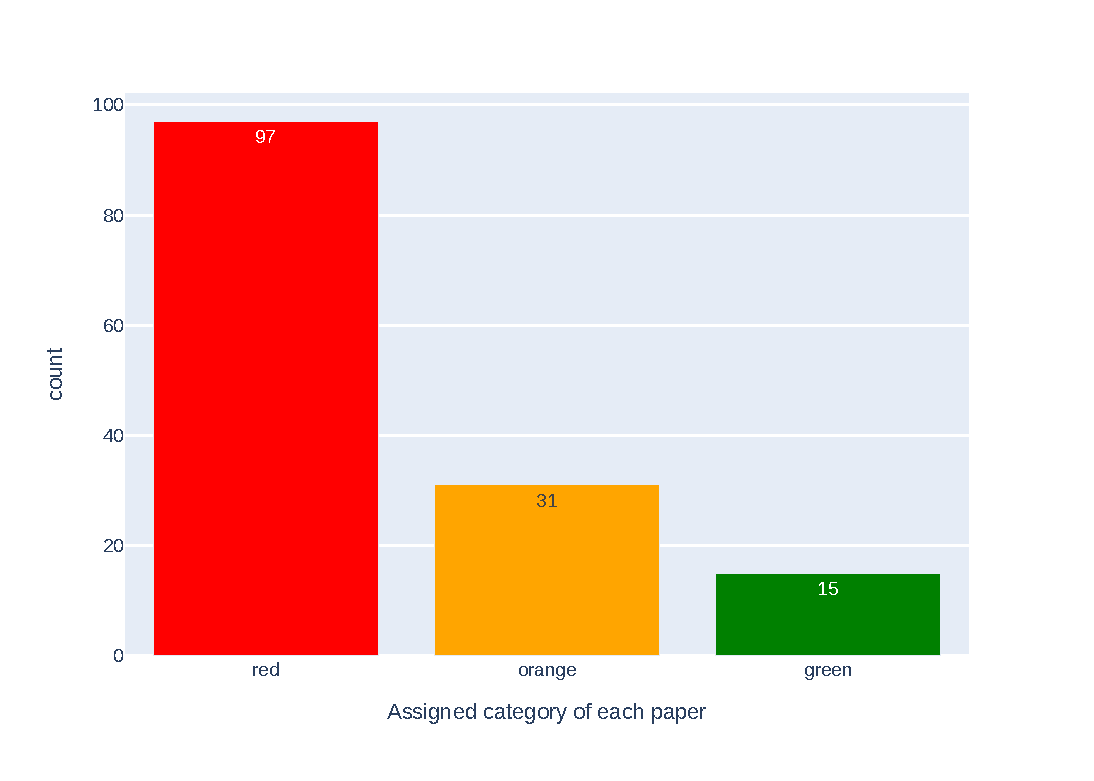
\includegraphics[width=\linewidth]{literaturrecherche/literature_study.pdf}
    \caption[short]{Results of the literature study}
    \label{fig:literature_study}
\end{figure}

Overall, through this approach, a lot of unrelated papers were found.
Nevertheless, with the 15 papers marked \emph{green}, the current state of carbon aware scheduling can be highlighted.
Out of those, the following are of particular interest.

\subparagraph{GreenSlot: Scheduling energy consumption in green datacenters\cite{inigo_goiri_greenslot_2011}} According to the analyzed papers, this seems to be the first paper that deals with carbon aware scheduling by implementing it as a \emph{Slurm} plugin (See section \ref{subsec:slurm_plugin} for further information on Slurm and such plugins)
In contrast to our scenario, where we try to optimize carbon emissions via the public electricity grid, GreenSlot is about datacenters having their own renewable energy production (e.g. via having solar panels on the roof). 
Using weather data, \emph{GreenSlot} predicts when solar energy production is high, scheduling jobs preferably in those time frames.
Under their workload model, jobs may also have deadlines.
If those deadlines cannot be met using only renewables, \emph{Greenslot} will additionally schedule jobs on high-carbon times, based on electricity cost.

\subparagraph{The War of the Efficiencies: the Tension between Carbon and Energy Optimization}\cite{hanafy_war_2023} This paper outlines the different ways of carbon aware computing. 
Among those are \emph{temporal shifting}, the idea that jobs can be executed later when energy is more carbon efficient, is also the main idea for my work. 
They also use \emph{spatial shifting}, moving jobs across the globe to areas where higher carbon efficiency is possible. 
\emph{Resource scaling} uses dynamic amounts of hardware according to carbon emissions.
In the end, \emph{rate shifting} is the idea to also scale hardware frequencies. During carbon-efficient times, CPU speeds are increased, leading to faster processing speeds and more energy usage.

All of these techniques are then tested under various parameters. My work will only make use of the temporal shifting, and abstract away the other methods of further carbon savings.

\subparagraph{Let's wait awhile: how temporal workload shifting can reduce carbon emissions in the cloud} This paper will be built upon in my work.\todo{Weigh this sentences with the GAIA paper as that is the one I am actually forking from}
The authors \cite{wiesner_lets_2021} use a simulation approach, to simulate temporal shifting. Their workload model consists of known length jobs that can use \emph{checkpoint \& restore} to be executed at different time slices. 
They further use different traces and test these traces under the assumption of different job-deadlines, meaning that each job has to be completed by a certain timeframe, and also different regions of the world as described in the background part\todo{Think about linking this to the earlier part}. 
Their main takeaways are that increased deadlines lead to reduced carbon emissions, but that this effect also has diminishing returns. 
They also deduced that regions such as California, with high amounts of solar power, have higher potential for carbon-savings in comparison to nuclear-heavy regions such as France.